% =================================================
% Chapter 6 — Final System Design and Design Summary
% =================================================

\section{Final System Design and Design Summary}

% -------------------------------------------------
\subsection{Final System Design}
% -------------------------------------------------

Following completion of the hydraulic analysis, pump selection, and wet well sizing, the wastewater conveyance system for the Colebrooke Subdivision is finalized as an integrated lift station and force main arrangement. The system consists of a duplex submersible pump station discharging through a short pressurized force main to the existing municipal gravity sewer manhole located along Lewis Street. The proposed pump station location, force main alignment, and downstream sewer connection were established using the subdivision survey and layout information \cite{ProjectD_Colebrooke_2020}.

The final arrangement of the pump station and force main is shown in Figure~\ref{fig:final_forcemain_layout}.

\begin{figure}[H]
\centering
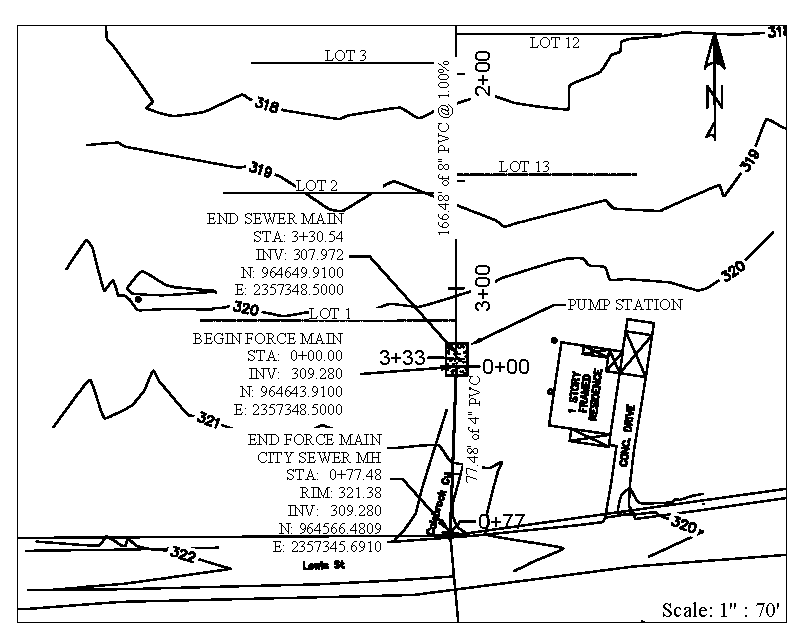
\includegraphics[
width=\textwidth
]{ForcemainLayoutPlan.pdf}
\caption{Final force main layout plan showing pump station location, 4-in force main alignment, and discharge connection to the existing city sewer manhole.}
\label{fig:final_forcemain_layout}
\end{figure}

As illustrated in Figure~\ref{fig:final_forcemain_layout}, the force main begins at the proposed pump station at Sta.~0+00.00 and extends approximately $77.48~\text{ft}$ to the existing municipal manhole at Sta.~0+77.48. The pump station coordinates are $N=964649.9100$, $E=2357348.5000$, and the receiving city sewer manhole is located at $N=964566.4809$, $E=2357345.6910$. Wastewater discharged from the pump enters the municipal gravity system at invert elevation $309.280~\text{ft}$.

The hydraulic relationship between the wet well and the receiving sewer is illustrated in Figure~\ref{fig:forcemain_profile}.

\begin{figure}[H]
\centering
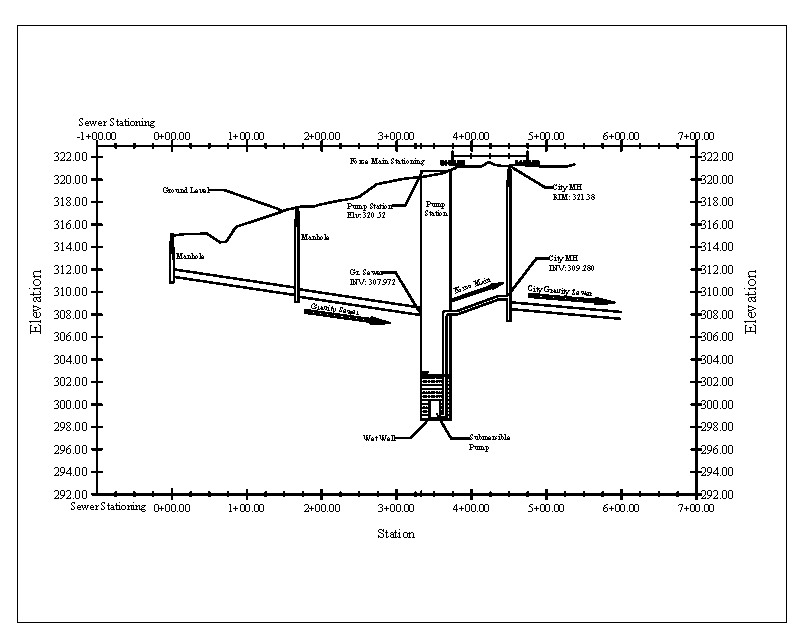
\includegraphics[
width=\textwidth
]{ForceMainLayoutProfile.pdf}
\caption{Final hydraulic profile showing the wet well, force main, and receiving city gravity sewer manhole.}
\label{fig:forcemain_profile}
\end{figure}

As shown in Figure~\ref{fig:forcemain_profile}, the wet well operating level is $299.00~\text{ft}$, while the receiving sewer invert is $309.280~\text{ft}$, producing a static head of $10.28~\text{ft}$. The profile confirms the short pressurized reach between the pump station and the municipal sewer connection and establishes the final vertical relationship between the wet well, ground surface, and discharge location.

% -------------------------------------------------
\subsection{Force Main Final Size Verification}
% -------------------------------------------------

The final force main diameter adopted for the system is $4$-in PVC pressure pipe. This size was selected after evaluating potential pipe diameters and confirming compliance with velocity, headloss, and regulatory requirements. Although the subdivision inflow is relatively small ($12.46~\text{gpm}$), wastewater lift stations using submersible pumps typically require a minimum $4$-in force main diameter except in grinder pump applications.

The final verification was performed using the selected pump operating point rather than the raw sewer inflow. The selected Sulzer XFP100C VX pump operates at $135.5~\text{gpm}$ and $12.08~\text{ft}$ of head according to the manufacturer performance curve. Using the pipe cross-sectional area of approximately $0.09~\text{ft}^2$, the resulting operating velocity is

\[
Q = 135.5~\text{gpm} = \frac{135.5}{448.83} = 0.302~\text{cfs}
\]

\[
V = \frac{Q}{A} = \frac{0.302}{0.09} = 3.36~\text{ft/s}
\]

\[
V \approx 3.4~\text{ft/s}
\]

This velocity exceeds the minimum wastewater transport velocity of $2~\text{ft/s}$ and falls within the commonly recommended $3$--$9~\text{ft/s}$ range for wastewater force mains. The value is sufficiently high to prevent solids deposition while remaining low enough to limit excessive headloss and pipe wear.

The total dynamic head corresponding to the selected pump operating point is $12.08~\text{ft}$, only slightly greater than the static head of $10.28~\text{ft}$, confirming that friction and minor losses remain small due to the short pipeline length and smooth PVC pipe surface.

The final force main configuration is therefore confirmed as

\[
\boxed{\text{4-in PVC force main, } L = 77.48~\text{ft}}
\]

% -------------------------------------------------
\subsection{Pump Station Configuration}
% -------------------------------------------------

The finalized lift station is configured as a duplex submersible sewage pumping station. The selected pump model is the Sulzer XFP100C VX 1$\sim$ (wet pit) equipped with a PE18/4W motor. The pump operates at $135.5~\text{gpm}$ and $12.08~\text{ft}$ of head, with a vortex impeller, DN100 suction outlet, DN100 discharge outlet, $3.94$-in free solids passage, and $2.414~\text{hp}$ motor output.

Two identical pumps are installed in the wet well. Under normal conditions one pump operates as the duty pump, while the second pump remains on standby. The standby pump provides redundancy and can automatically start if the inflow exceeds the capacity of a single pump or if the duty pump becomes unavailable. This configuration improves reliability and is standard practice for small municipal wastewater lift stations.

The selected pump uses a vortex impeller, which allows solids and fibrous material to pass through the pump casing without direct contact with the impeller vanes. This configuration improves clogging resistance for residential wastewater systems. The manufacturer data indicate a $3.94$-in free passage, which exceeds the typical $3$-in solids-handling requirement commonly used in wastewater pump selection.

% -------------------------------------------------
\subsection{Pump Station Control Levels}
% -------------------------------------------------

Once the wet well diameter and storage volume were determined, the control elevations governing pump operation were established. The control hierarchy consists of minimum submergence, active storage depth, lag-pump storage, and reservoir storage.

The finalized control elevation arrangement is illustrated in Figure~\ref{fig:final_wetwell_levels}.

\begin{figure}[H]
\centering
\includegraphics[
width=\textwidth,
page=2,
trim={1.5in 2.5in 1in 4in},
clip
]{forcemain_pump_figures.pdf}
\caption{Wet well control elevations showing minimum submergence, storage depth, lag pump activation, and high-water alarm levels.}
\label{fig:final_wetwell_levels}
\end{figure}

As shown in Figure~\ref{fig:final_wetwell_levels}, the final control increments are

\begin{enumerate}
\item Minimum submergence ($H_x = 14$ in)
\item Pump-off to lead-pump-on storage ($H_{min} = 14.2$ in)
\item Lead-pump-on to lag-pump-on storage ($H_{lag} = 6$ in)
\item Lag-pump-on to high-water alarm storage ($H_{res} = 12$ in)
\end{enumerate}

The minimum submergence between the pump inlet and pump-off water level was determined using the Hecker relation

\[
H_x = D(1+2.3F_D)
\]

with

\[
F_D = \frac{V}{\sqrt{gD}}
\]

Using the DN100 suction diameter and the pump operating flow, the required submergence was calculated as

\[
H_x = 13.9~\text{in} \approx 14~\text{in}
\]

The active storage depth was determined from the selected wet well storage volume of $250~\text{gal}$ and a $6$-ft diameter wet well, giving a cross-sectional area of $28.27~\text{ft}^2$. Converting storage volume to cubic feet,

\[
V = 250(0.13368) = 33.42~\text{ft}^3
\]

\[
H_{min} = \frac{V}{A} = \frac{33.42}{28.27} = 1.18~\text{ft} = 14.2~\text{in}
\]

These values establish the final pump control elevations summarized in Table~\ref{tab:control_levels}.

\begin{table}[H]
\centering
\caption{Final wet well control elevations}
\label{tab:control_levels}
\begin{tabular}{lc}
\toprule
Control increment & Value \\
\midrule
Minimum submergence ($H_x$) & 14 in \\
Pump-off to lead-pump-on ($H_{min}$) & 14.2 in \\
Lead-pump-on to lag-pump-on ($H_{lag}$) & 6 in \\
Lag-pump-on to high-water alarm ($H_{res}$) & 12 in \\
\bottomrule
\end{tabular}
\end{table}

% -------------------------------------------------
\subsection{Accessories and Mechanical Components}
% -------------------------------------------------

In addition to the pumps themselves, several mechanical components are required to support installation, maintenance, and operation of the lift station. These include guide rails, duckfoot discharge elbows, discharge piping, valves, and access openings.

The installation arrangement for the selected pump is illustrated in Figure~\ref{fig:sulzer_install}.

\begin{figure}[H]
\centering
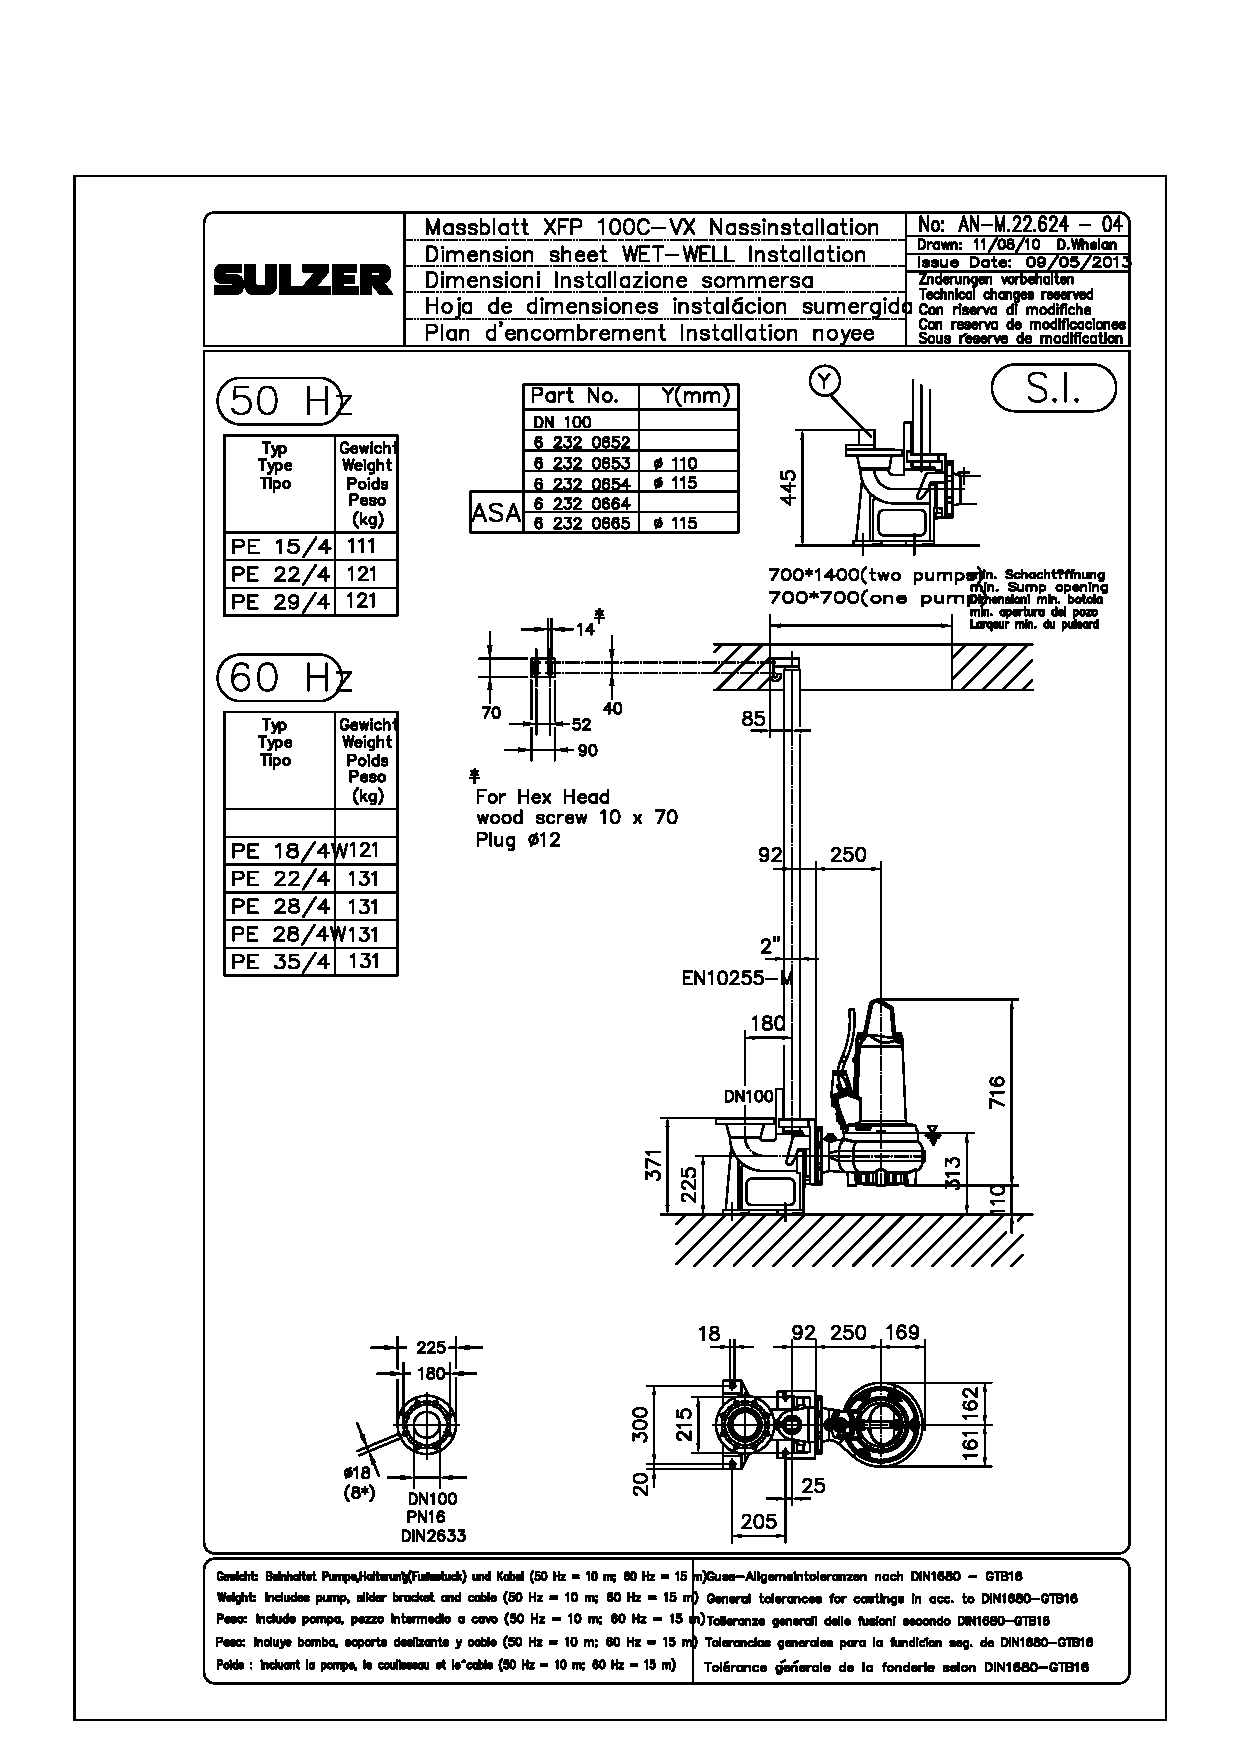
\includegraphics[
width=0.9\textwidth
]{dimension_ANM22624.pdf}
\caption{Sulzer XFP100C VX wet well installation arrangement showing duplex hatch opening, guide rail system, and discharge connection details.}
\label{fig:sulzer_install}
\end{figure}

Each pump is mounted on a guide rail system that allows removal and reinstallation from the ground surface without entering the wet well. The pumps connect to duckfoot discharge elbows at the base of the wet well, directing flow into the vertical discharge piping.

The manufacturer installation sheet indicates a recommended duplex hatch opening of $28~\text{in} \times 56~\text{in}$, which was adopted in the wet well design. The installation drawing also confirms the use of $4$-in Class 125 ANSI discharge hardware associated with the DN100 pump connection.

The discharge piping includes both a check valve and gate valve. The check valve prevents reverse flow when pump operation stops, while the gate valve allows isolation of the discharge piping during maintenance. Additional station components include lifting chains, level sensors, electrical power connections, and control equipment necessary for automatic pump operation.

% -------------------------------------------------
\subsection{Final Design Summary}
% -------------------------------------------------

The final design for the Colebrooke Subdivision lift station integrates the subdivision gravity sewer system with the existing municipal sewer network through a short pressurized force main and duplex wet well pump station. Wastewater collected from the subdivision flows to the wet well at a peak rate of $12.46~\text{gpm}$ and is pumped through a $4$-in PVC force main approximately $77.48~\text{ft}$ in length to the existing city sewer manhole at invert elevation $309.280~\text{ft}$ \cite{ProjectD_Colebrooke_2020}.

The selected pump is the Sulzer XFP100C VX 1$\sim$ (wet pit) with vortex impeller, operating at $135.5~\text{gpm}$ and $12.08~\text{ft}$ of head with $1.765~\text{hp}$ shaft power and $2.414~\text{hp}$ motor output. The wet well is designed as a $6$-ft inside diameter circular structure with $250~\text{gal}$ active storage, providing adequate storage and stable pump cycling.

The key design parameters are summarized in Table~\ref{tab:design_summary}.

\begin{table}[H]
\centering
\caption{Final system design summary}
\label{tab:design_summary}
\begin{tabular}{lc}
\toprule
Item & Final design \\
\midrule
Peak wastewater inflow & 12.46 gpm \\
Selected pump model & Sulzer XFP100C VX \\
Pump operating flow & 135.5 gpm \\
Pump operating head & 12.08 ft \\
Impeller type & Vortex \\
Free passage & 3.94 in \\
Motor output & 2.414 hp \\
Force main material & PVC pressure pipe \\
Force main diameter & 4 in \\
Force main length & 77.48 ft \\
Static head & 10.28 ft \\
Total dynamic head & 12.08 ft \\
Wet well diameter & 6 ft \\
Active wet well storage & 250 gal \\
Hatch opening & 28 in $\times$ 56 in \\
$H_x$ & 14 in \\
$H_{min}$ & 14.2 in \\
$H_{lag}$ & 6 in \\
$H_{res}$ & 12 in \\
\bottomrule
\end{tabular}
\end{table}

The final design satisfies the hydraulic requirements of the subdivision and provides adequate solids-handling capability and operational reliability. The selected pump, wet well, and force main operate as an integrated system consistent with the project layout and manufacturer installation requirements \cite{ProjectD_Colebrooke_2020}.
